\documentclass[letterpaper,11pt]{article}
\usepackage{science}
\usepackage[utf8]{inputenc}
\usepackage{mathtools}
\usepackage{subcaption}
\usepackage{tikz}
\usepackage{pgf}
\usepackage{pgfplots}
\usepackage{circuitikz}

\title{\textbf{Transistor bipolare:} interruttore}
\author{Canteri Marco, Biasi Lorenzo, Damiani Emily}
\date{\today}

\begin{document}
\maketitle

\begin{abstract}
\hspace{-1.5em}Abbiamo studiato il funzionamento di un transistor utilizzato come interruttore, analizzandone la zona di saturazione e di interdizione. In seguito abbiamo utilizzato tale transistor collegato ad un generatore di onda quadrata per costruire un interruttore per far lampeggiare un LED con frequeza a scelta.
\end{abstract}

\begin{body}
\section{Obiettivi}
\begin{itemize}
\item Studiare il funzionamento di un transistor bipolare come interruttore.
\item Analizzare il circuito interruttore transistor, compresa la condizione di saturazione della
corrente collettore.
\end{itemize}
\section{Procedimento}
È stato costruito il circuito in figura \eqref{circuito1}, dove $R_c = 1001 \pm \Omega$, $R_b$ decade variabile e come sorgente di potenziale $V=15 V$. Variando la resistenza $R_b$ nel circuito di controllo del transistor si può far variare la corrente di base che entra nel transistor, è stata quindi misurata la corrente $i_c$ con il generatore di $V$, con il multimetro si è misurata la corrente $i_b$ e sempre col multimetro si è misurata la differenza di potenziale ai capi del collettore e dell'emissore del transistor $V_{ce}$.
Abbiamo poi costruito il circuito in figura \eqref{circuito2}, collegando la base del transistor a un generatore d'onda quadra, $R_b$ è stata fissata a $10 \text{k}\Omega$. In questo modo si è costruito un interruttore veloce con frequenza a piacimento. Il segnale di controllo $V_{in}$ del transistor è un onda quadra variabile tra 0 e 5 $V$

\begin{figurehere}
\begin{subfigure}[H]{0.2\textwidth}
\begin{circuitikz}
\draw (0,0) node[ground, rotate=180]{} to [battery, l=$V$] (0,-1.5)
to [R=$R_c$] (0,-3)
to [leD*] (0,-4.5);
\draw
(0,-5.0) node[npn] (npn) {}
(npn.emitter) node[ground]{};
\draw (0,-1.5)
to [short] (-1.5,-1.5)
to [ospst] (-1.5,-3)
to [R=$R_b$] (-1.5,-5.0)
to [short] (npn.base);
\end{circuitikz}
\caption{Transistor come interruttore}\label{circuito1}
\end{subfigure}
\hfill
\begin{subfigure}[H]{0.2\textwidth}
\begin{circuitikz}[scale=0.82]
\draw (0,0) node[ground, rotate=180]{} to [battery, l=$V$] (0,-1.5)
to [R=$R_c$] (0,-3)
to [leD*] (0,-4.5);
\draw
(0,-5.0) node[npn] (npn) {}
(npn.emitter) node[ground]{};
\draw (-3,-7)node[ground]{}
to [sqV, l =$V_{in}$] (-3,-5)
to [R=$R_b$] (npn.base);
\end{circuitikz}
\caption{Transistor con interruttore veloce}\label{circuito2}
\end{subfigure}
\end{figurehere}
\section{Analisi dati}
Con l'interruttore chiuso abbiamo variato la resistenza $R_b$ e misurato le correnti, con l'obbiettivo di cercare la minima corrente $i_b$ di saturazione del transistor, ovvero quando la tensione $V_{ce}$, 
dove quindi il transistor funziona come corto circuito. In questa condizione la corrente $i_c$ che scorre nel transistor è indipendente dalla corrente $i_b$ della base.  
\newpage
\begin{figurehere}
\centering
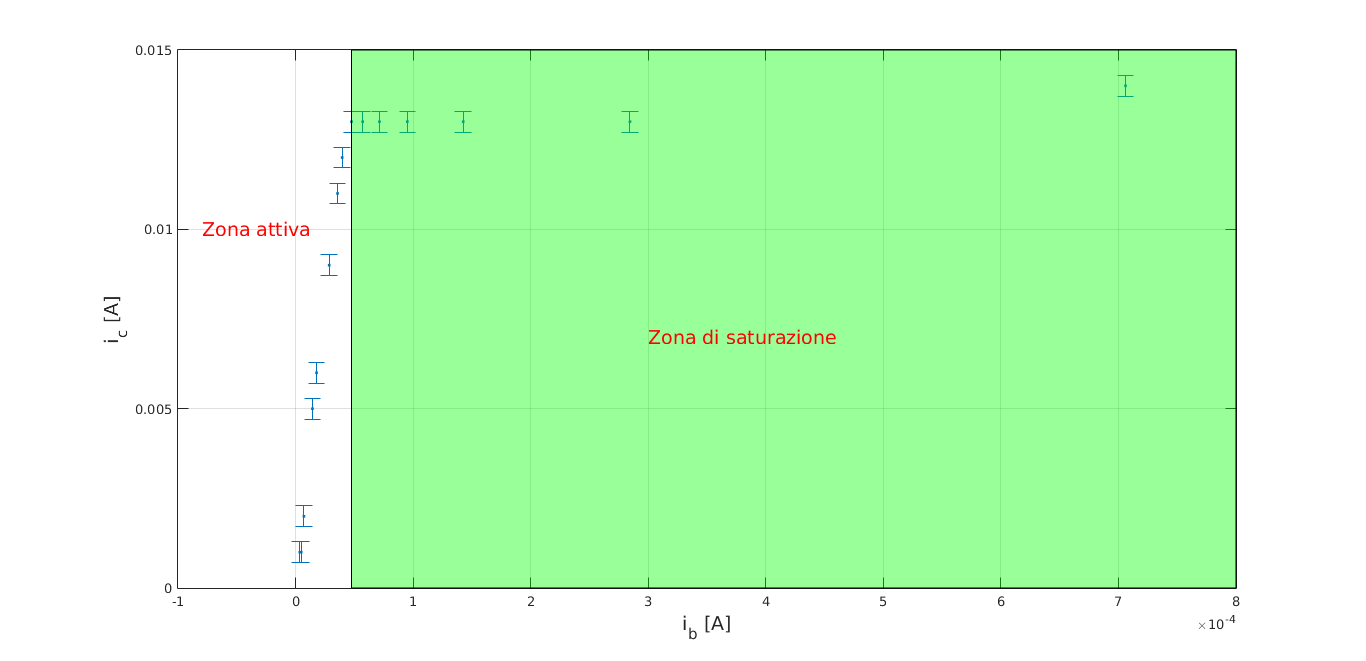
\includegraphics[width=0.5\textwidth]{sat.png}
\caption{Zona di saturazione e zona attiva del transistor}
\end{figurehere}
\end{body}
\end{document}
